\section{Zielsetzung}
In diesem Versuch wird das Relaxationsverhalten des RC-Kreises untersucht. 
Dazu werden Größen wie die Zeitkonstante, Amplituden der Kondensatorspannung und Phasenverschiebungen gemessen.

\section{Theoretische Grundlagen}

\noindent
Eine Relaxationserscheinung tritt auf, wenn ein System aus seinem Ausgangszustand entfernt wird und es nicht-oszillatorisch in den Ausgangszustand zurückkehrt.
Wird eine Größe A betrachtet, lässt sich ihre Änderungsgeschwindigkeit zum Zeitpunkt t darstellen als:

\begin{equation}
\frac{\text{dA}}{\text{dt}}=\text{c} [ \text{A} ( \text{t} ) - \text{A} ( \text{\infty} ) ]  .
\end{equation}

\noindent
Durch Integration vom Zeitpunkt 0 bis t und umstellen ergibt sich dann 

\begin{equation}
\text{A} ( \text{t} ) = \text{A} ( \text{\infty} ) + [ \text{A} ( 0 ) - \text{A} ( \text{\infty} ) ] \, \symup{e}^\text{ct}
\label{eqn:e}  
\end{equation}

\noindent
mit $\text{c}<0$.

\noindent
Die Ent- und Aufladevorgänge eines Kondensators über einen Widerstand sind Beispiele für Relaxationsvorgänge, die im Folgenden näher untersucht werden.

\noindent
\begin{figure}
            \centering
               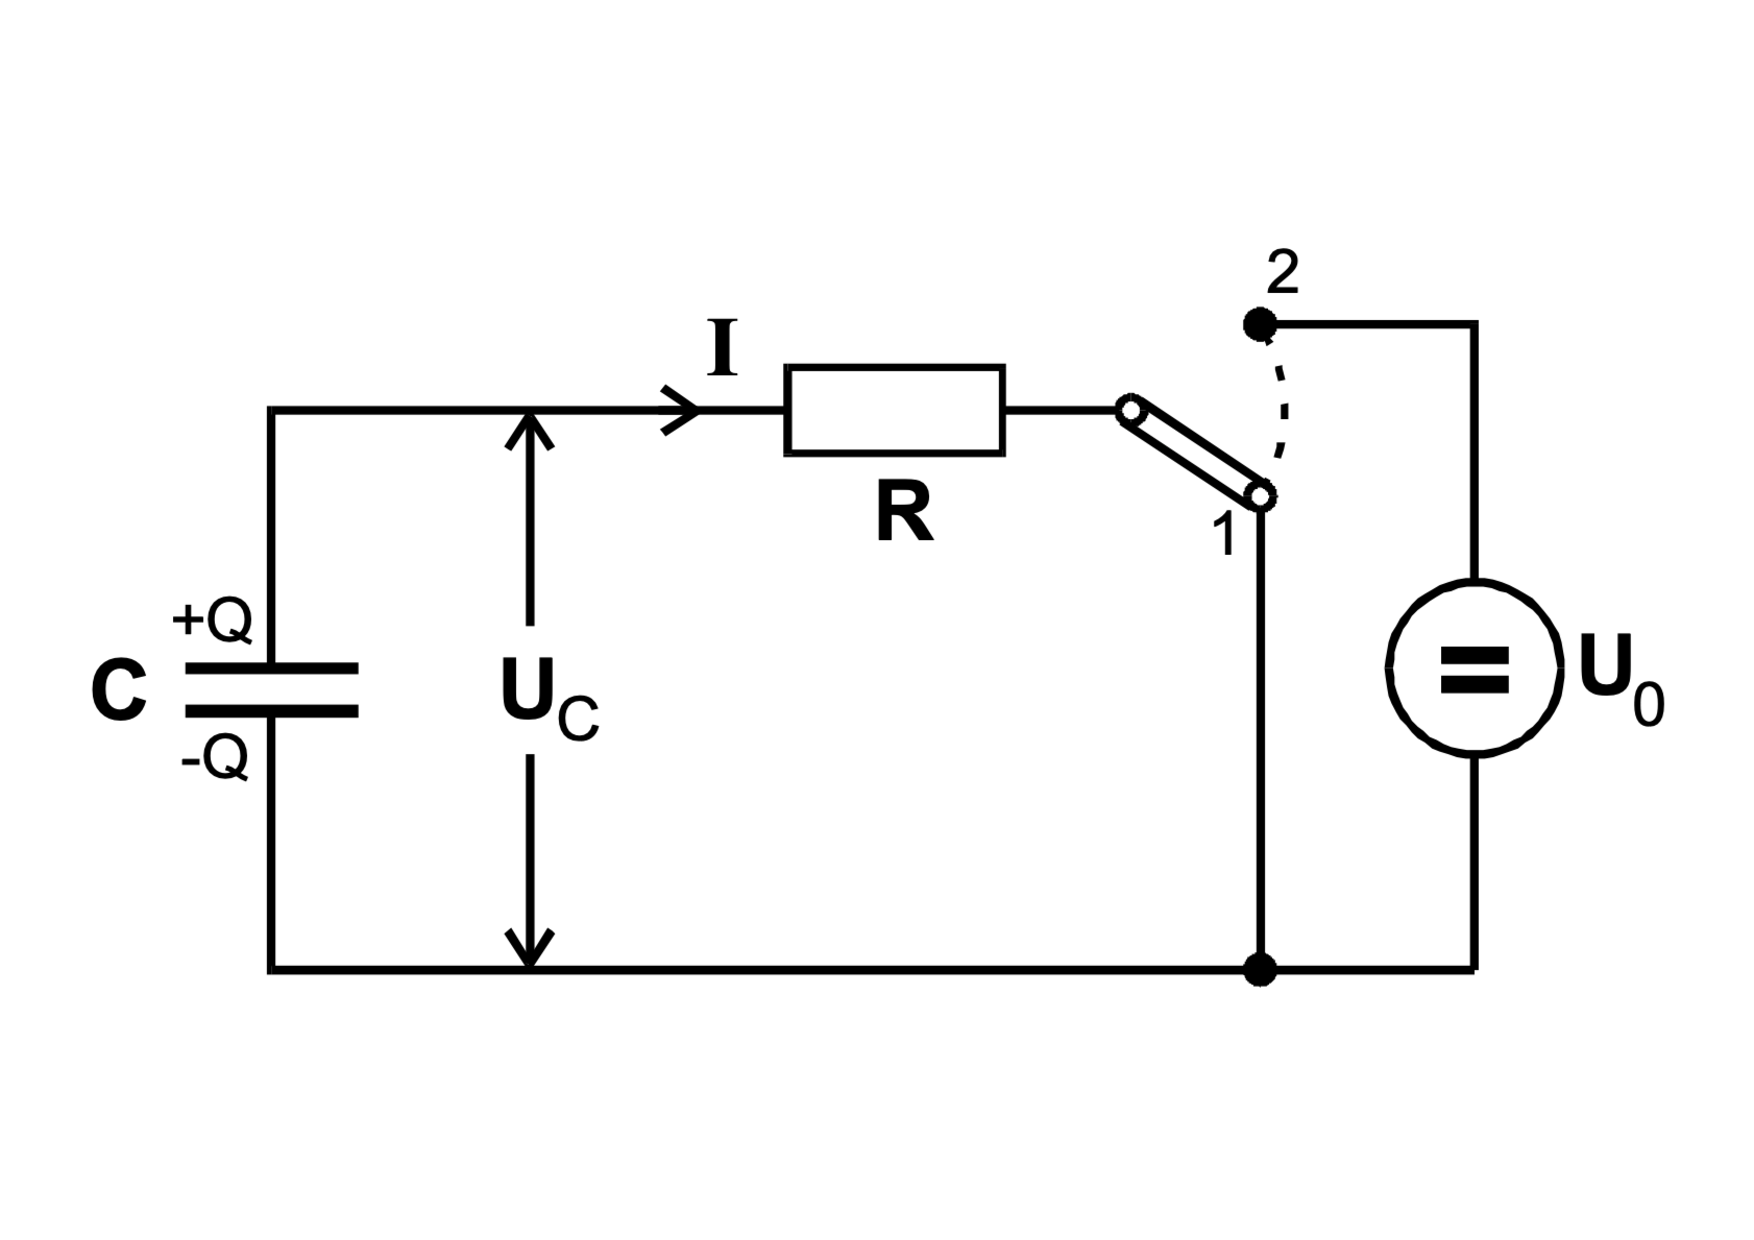
\includegraphics[height=5cm]{rc.pdf}
               \caption{Entladung (1) und Aufladung (2) eines Kondensators über einen Widerstand.}
               \label{fig:rc}
\end{figure}

\begin{enumerate}
\item \textbf{Entladevorgang}

Auf den Platten eines Kondensators mit der Kapazizät C und der Ladung Q ist die Spannung zwischen ihnen durch

\begin{equation}
\text{U}_\text{C}=\frac{\text{Q}}{\text{C}}
\label{eqn:u}
\end{equation}

gegeben.
Mit

\begin{equation}
\text{I}=\frac{\text{U}_\text{C}}{\text{R}}
\label{eqn:i}
\end{equation}

und

\begin{equation}
\text{dQ}=-\text{Idt}
\label{eqn:dq}
\end{equation}

lässt sich nun eine Differentialgleichung für den zeitlichen Verlauf der Ladung auf dem Plattenkondensator aufstellen.

\begin{equation}
\frac{\text{dQ}}{\text{dt}}=-\frac{1}{\text{RC}} \text{Q}(\text{t})
\label{eqn:dgl}
\end{equation}

Mit der Randbedingung 

\begin{equation}
\text{Q}(\infty)=0
\end{equation}

lässt sich die DGL (\ref{eqn:dgl}) lösen zu

\begin{equation}
\text{Q}(\text{t}) = \text{Q}(0) \symup{e}^{-\frac{\text{t}}{\text{RC}}}.
\end{equation}

\item \textbf{Aufladevorgang}

Mit den Randbedingungen für den Aufladevorgang

\begin{equation}
\text{Q}(\infty)=\text{CU}_0
\end{equation}

und 

\begin{equation}
\text{Q}(0)=0
\end{equation}


lässt sich die DGL (\ref{eqn:dgl}) lösen zu

\begin{equation}
\text{Q}(\text{t}) = \text{CU}_0 (1 - \symup{e}^{-\frac{\text{t}}{\text{RC}}}).
\end{equation}

Dabei ist der Ausdruck RC die Zeitkonstante, die angibt, wie schnell das System seinen Endzustand Q($\infty$) anstrebt.
Das bedeutet, dass sich pro Zeitraum $\Delta$T=RC die Ladung auf dem Plattenkondensator und den Faktor

\begin{equation}
\frac{\text{Q}(\text{t}=\text{RC})}{\text{Q}(0)} = \frac{1}{\text{e}}
\end{equation}

ändert.

\end{enumerate}

\newpage
\noindent
\textbf{Relaxationsphänomene, die unter dem Einfluss einer periodischen Auslenkung aus der Gleichgewichtslage auftreten}

\noindent
Nun wird das Relaxationsphänomen auf einen RC-Kreis mit Wechselspannung nach Abbildung (\ref{fig:rcwechsel})betrachtet.

\begin{figure}
            \centering
               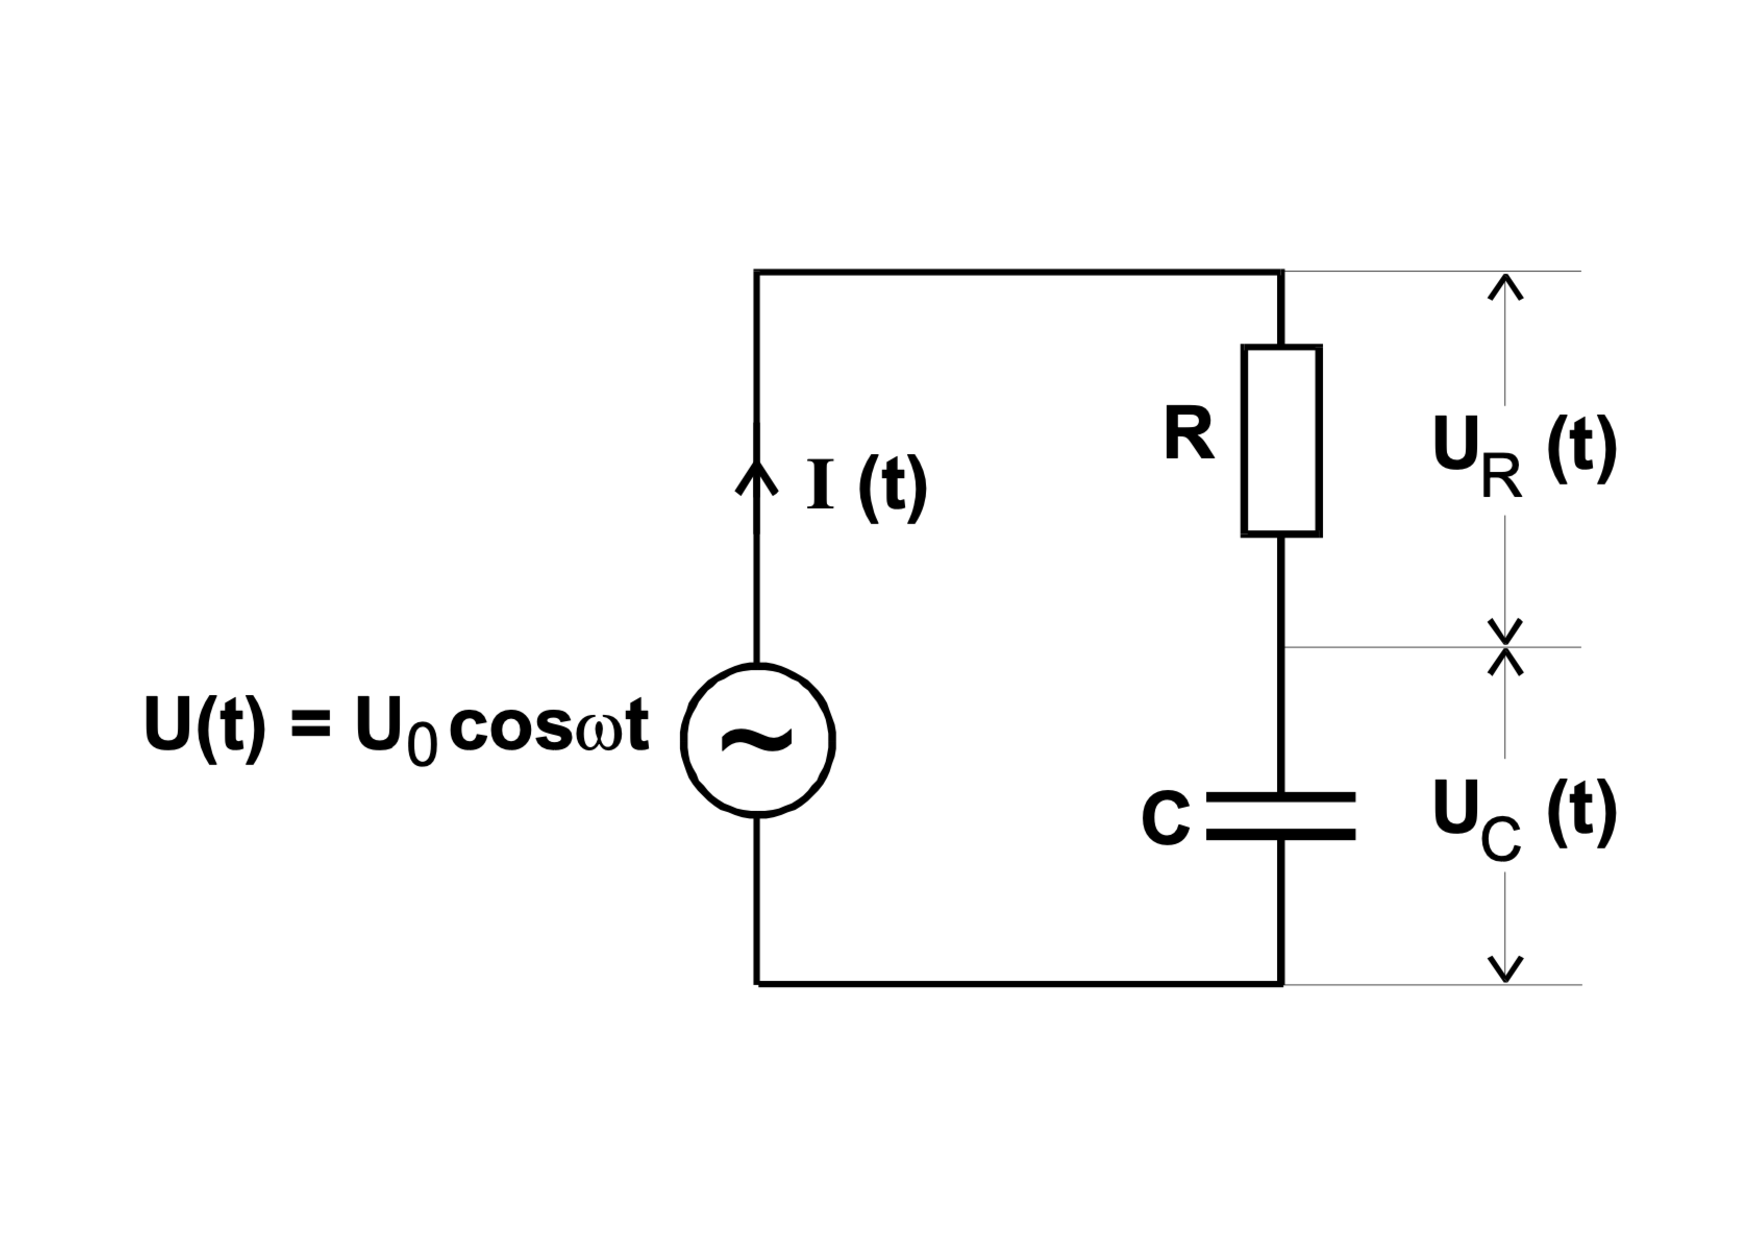
\includegraphics[height=5cm]{rcwechsel.pdf}
               \caption{RC-Kreis mit Wechselspannung.}
               \label{fig:rcwechsel}
\end{figure}

\noindent
Wenn die Kreisfrequenz $\omega$ klein genug ist, also $\omega << \frac{1}{\text{RC}}$ gilt, kann angenommen werden, dass $\text{U}(\text{t}) = \text{U}_\text{C}$ gilt.
Mit zumehmender Frequenz tritt eine Phasenverschiebung $\phi$ zwischen den Spannungen $\text{U}(\text{t})$ und $\text{U}_\text{C}$ auf, da die Ent- und aufladung des Kondensators zeitlich hinter der äußeren Spannung zurück bleibt.
Mit der Amplitude A ergibt sich der Ansatz:

\begin{equation}
\text{U}_\text{C} (\text{t}) = \text{A} (\omega) \text{cos}(\omega\text{t} + \phi)
\end{equation}

\noindent
Mithilfe des Maschensatzes lässt sich aus Abbildung (\ref{fig:rcwechsel}) folgender Ausdruck formulieren:

\begin{equation}
\text{U}_0 \text{cos}(\omega \text{t}) = \text{I}(\text{t})\text{R} + \text{A} (\omega) \text{cos}(\omega\text{t} + \phi).
\label{eqn:masch}
\end{equation}

\noindent
Mit Gleichung (\ref{eqn:u}) und (\ref{eqn:dq}) kann I(t) umgeschrieben werden zu

\begin{equation}
\text{I}(\text{t}) = \text{C} \frac{\text{dU}_\text{C}}{\text{dt}}
\label{eqn:it}
\end{equation}

\noindent 
und kann in (\ref{eqn:masch}) eingesetzt werden.
Daraus ergibt sich:

\begin{equation}
\text{U}_0 \, \text{cos}(\omega \text{t}) = -\text{A}\omega\text{RC} \, \text{sin} (\omega\text{t} + \phi ) + \text{A} (\omega) \, \text{cos}(\omega\text{t} + \phi).
\label{eqn:u0}
\end{equation}

\noindent
Wird nun $\omega \text{t} = \frac{\pi}{2}$ gewählt und ausgenuntzt, dass $\text{sin}(\frac{\pi}{2} + \phi) = \text{cos}(\phi)$ und $\text{cos}(\frac{\pi}{2} + \phi) = -\text{sin}(\phi)$ gilt, folgt aus Gleichung (\ref{eqn:u0})

\begin{equation}
0 = -\text{A}\omega\text{RC}\, \text{cos}(\phi) - \text{A} (\omega) \, \text{sin}(\phi) \\
\iff \phi = \text{arctan}(-\omega\text{RC})
\label{eqn:phi}
\end{equation}

\noindent
Weiter folgt aus (\ref{eqn:u0}) für $\omega\text{t} + \phi = \frac{\pi}{2}$

\begin{equation}
\text{U}_0 \, \text{cos}(\frac{\pi}{2} - \phi) = -\text{A}\omega\text{RC}
\iff \text{A}(\omega) = - \frac{\text{sin} \, \phi}{\omega\text{RC}} \text{U}_0
\label{eqn:a}
\end{equation}

\noindent
Wird nun Gleichung (\ref{eqn:phi}) weiter umgeformt zu 

\begin{equation}
\text{sin} \, \phi = \frac{\omega \text{RC}}{\sqrt{1 + \omega^2 \text{R}^2 \text{C}^2 }}
\end{equation}

\noindent
kann dieser Ausdruck in Gleichung (\ref{eqn:a}) eingesetzt werden. Daraus ergibt sich 

\begin{equation}
\text{A}(\omega) = \frac{\text{U}_0}{\sqrt{1 + \omega^2 \text{R}^2 \text{C}^2 }}
\label{eqn:sqrt}
\end{equation}

\noindent
Unter bestimmten Vorraussetzungen ist es möglich, eine zeitlich veränderte Spannung in einem wie in Abbildung (\ref{fig:rcwechsel}) gezeigten System zu Integrieren.
Zunächst wird die Maschenregel auf die in Abbildung (\ref{fig:rcwechsel}) gezeigte Schaltung angewendet. Daraus folgt:

\begin{equation}
\text{U}(\text{t}) = \text{I}(\text{t})\text{R} + \text{U}_\text{C}.
\end{equation}

\noindent
Nun wird für $\text{I}(\text{t})$ der Ausdruck aus Gleichung (\ref{eqn:it}) eingesetzt.

\begin{equation}
\text{U}(\text{t}) = \text{RC} \frac{\text{dU}_\text{C}}{\text{dt}} + \text{U}_\text{C}.
\label{eqn:utt}
\end{equation}

\noindent
Unter der Vorraussetzung, dass $\omega >> \frac{1}{\text{RC}}$ gilt, ist $|\text{U}_\text{C}| << |\text{U}_\text{R}|$ und  $|\text{U}_\text{C}| << |\text{U}|$
Näherungsweise kann die Gleichung (\ref{eqn:utt}) nun vereinfacht werden zu

\begin{equation}
\text{U}(\text{t}) = \text{RC} \frac{\text{dU}_\text{C}}{\text{dt}}.
\end{equation}

\noindent
Umgestellt nach $\text{U}_\text{C}$ ergibt dies

\begin{equation}
\text{U}_\text{C} = \frac{1}{\text{RC}} \int_0^\text{t} \text{U}(\text{t'}) \text{dt'}
\label{eqn:int}
\end{equation}

\noindent
Gleichung (\ref{eqn:int}) ist zu entnehmen, dass $\text{U}_\text{C}$ proportional zu $\int \text{U}(\text{t})$ ist, wenn $\omega >> \frac{1}{\text{RC}}$ gilt.
